\subsection{Object identification}
\label{sec:language-games:identification}

\subsubsection*{Setup}

The object identification game is set up as a discrimination game.
In a discrimination game, the agents are presented with two or more images, one of these being the target image.
The sender needs to communicate this target image to the receiver by discriminating it from the other distractor images.
The receiver then needs to decide based on the message, which of the images is the target image.

The discrimination games in this research have a very similar setup as described in \citep{Lazaridou2017}.
The agents in this research resemble their \emph{agnostic sender} as well as their \emph{receiver}.
One central difference is the production of the message.
The main goal of their language games was the identification of the concept that the shown image was related to.
Therefore, the sender communicated only single-symbol messages to the receiver which should describe the concept of the target image.
Opposed to that, in this research, the agents are tasked to discriminate objects from each other based on their attributes.
% SD: On the contrary,...
% DK: (done)
It is therefore assumed that the sender will communicate these discriminative attributes.
For that reason, the sender is allowed to generate sequences as a message where for instance each symbol in the sequence might correspond to one attribute.

The data is prepared in the same way as for the single model object identification task in section \ref{sec:object-identification}.
Bounding boxes of all objects in the scene are extracted and preprocessed to be used for the feature extractors.
For datasets with a variable number of objects, the list bounding of bounding boxes is padded with a matrix of zeros to the maximum possible number of objects present in a scene across the
dataset.
Opposed to the experiments with one neural model, no additional information about the target object's attributes is provided.
Instead, the sender agent is presented with the target object always as the first object, while the distractors are shuffled.
The receiver is presented with completely shuffled bounding boxes.

Accordingly, also the models from the single model tasks serve as basis for the object identification task.
The sender uses the architecture of the model described in section \ref{sec:referring_expression_generation} apart from the final LSTM.
Instead, it will use the LSTM with a hidden size $h_s$ included in the \emph{EGG} framework to produce a message.
Based on the results from the single model object identifiers, the image embedding size $e_s$ is fixed to 100.

The receiver instead uses the architecture of the single model object identifier, described in section \ref{sec:object-identification}.
Similarly to the sender, the LSTM of the \emph{EGG} framework with the hidden size $h_e$ is used to encode the sender's message instead of the one-hot encoded attributes in the single model.
The hidden state of the LSTM is projected to the embedding size $e_r=500$ with a linear layer, based on the results in the previous experiments.
As before the dot product between the embedded message and the encoded image is calculated to let the model point towards the bounding box that is described best by the message.
Figure \ref{fig:discriminator_architecture} shows, how the sender and the receiver of the discriminator are built up.

\begin{figure}[ht]
    \centering
    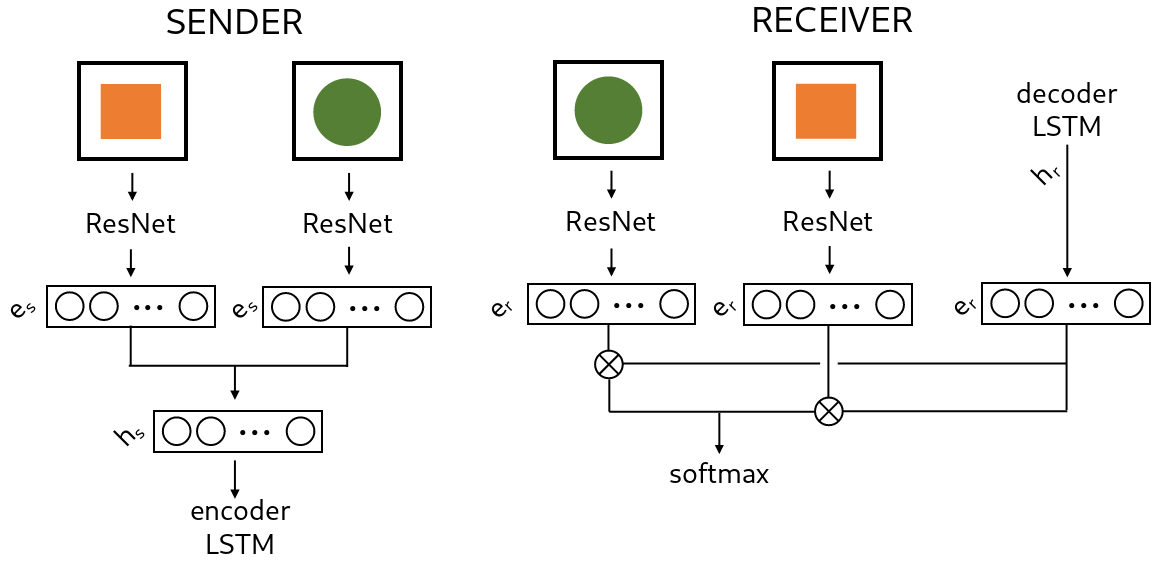
\includegraphics[width=.8\linewidth]{figures/arch_discriminator.png}
    \caption{Sender and receiver architectures in the discrimination game}
    \label{fig:discriminator_architecture}
\end{figure}

The experiments are conducted with a learning rate of $2\times10^{-4}$, the loss is calculated using cross entropy.
The following values for the variables are compared:
\begin{itemize}
    \item $h_s$: 100, 500, 1000
    \item $h_r$: 100, 500, 1000
    \item $|V|$: 2, 10, 16, 50, 100
    \item $n$: 1, 2, 3, 4, 6
\end{itemize}

The language game is run on the 'Dale-2', 'Dale-5' and 'CLEVR color' datasets.
A random guess corresponds to 50\% in the \emph{Dale-2} dataset, 20\% in the \emph{Dale-5} dataset and 13\% in the \emph{CLEVR color} dataset.

\subsubsection*{Results}
When looking at the results of the experiments, it can be seen that the agents are successfully discriminating the objects across all datasets.
Tables \ref{tab:results_discriminator_dale-2} to \ref{tab:results_discriminator_color} give an overview over the accuracy scores of selected configurations.
For each dataset there are many configurations that outperform the baseline models by a high margin.
However, there are still clear differences between the accuracy scores of each dataset.

\cmtDK[inline]{baseline}
\cmtDK[inline]{learning curve}
% SD: As we discussed at Semdial, it would be good to have a learning curves here that would show how fast or slow the languages converge. As David pointed out it may be that convergence is unstable and changes happen in between.
% DK: TODO

\begin{table}[ht]
    \centering
    \begin{tabular}{cccc|c}
        \toprule
                                      &           &     &       & \multicolumn{1}{c}{\textbf{Dale-2}} \\  \cmidrule(lr){5-5}
        $h_r$                         & $h_s$     & $n$ & $|V|$ & \textbf{Accuracy}                   \\\midrule
        {100}                         & {100}     & {2} & {10}  & {99,96\%}                           \\
        {100}                         & {1000}    & {2} & {10}  & {99,96\%}                           \\
        {1000}                        & {100}     & {3} & {10}  & {99,87\%}                           \\
        {500}                         & {100}     & {3} & {100} & {99,83\%}                           \\
        {100}                         & {100}     & {6} & {50}  & {99,83\%}                           \\
        {100}                         & {500}     & {3} & {16}  & {99,7\%}                            \\
        {1000}                        & {100}     & {6} & {16}  & {99,61\%}                           \\
        {100}                         & {100}     & {6} & {100} & {99,57\%}                           \\
        {100}                         & {500}     & {1} & {100} & {99,52\%}                           \\
        {100}                         & {100}     & {1} & {50}  & {99,35\%}                           \\
        {500}                         & {100}     & {1} & {2}   & {99,26\%}                           \\
        {100}                         & {500}     & {1} & {50}  & {99,26\%}                           \\
        {500}                         & {500}     & {1} & {100} & {99,26\%}                           \\
        {100}                         & {500}     & {3} & {100} & {99,83\%}                           \\
        {500}                         & {1000}    & {1} & {16}  & {98\%}                              \\
        {100}                         & {500}     & {1} & {10}  & {96,61\%}                           \\
        {100}                         & {1000}    & {1} & {100} & {99,44\%}                           \\
        {500}                         & {500}     & {6} & {2}   & {95,92\%}                           \\
        {100}                         & {1000}    & {4} & {2}   & {94,88\%}                           \\
        {100}                         & {1000}    & {6} & {10}  & {63,15\%}                           \\
        {1000}                        & {500}     & {2} & {2}   & {62,98\%}                           \\\midrule
        \multicolumn{4}{c|}{baseline} & {62,72\%}                                                     \\\midrule
        {100}                         & {1000}    & {3} & {2}   & {61,2\%}                            \\
        \bottomrule
    \end{tabular}
    \caption{Selected results of the object identification games on the Dale-2 dataset with $e_s=100$ and $e_r=500$}
    \label{tab:results_discriminator_dale-2}
\end{table}

When the agents are tasked to discriminate between the two objects of the \emph{Dale-2} dataset, it succeeds in almost all configurations with an accuracy of over 94\%.
Selected results are listed in Table \ref{tab:results_discriminator_dale-2}.
In many configurations the accuracy lies above 99\%, while only 4 configurations have an accuracy of only 61\% to 64\%.
An antecedent for a low accuracy seems to be a low vocabulary size $|V|$.
All experiments with a vocabulary size of only two symbols (including the <eos> symbol) tend to give worse results.
Three of the four results that don't surpass the baseline use a vocabulary size of 2.
On the other side, only few configurations with $|V| = 2$ are among the overall best results.
When the vocabulary size is increased, the results become better.
Especially configurations with $|V| = 10$, $|V| = 16$, $|V| = 50$ and $|V| = 100$ consistently achieve high accuracies.
While there are some few exceptions, the results show that the agents tend to perform better, when they can exchange messages with more than one symbol.
Hereby, even games with an $n = 6$ perform as well as games with $n = 2$ as seen for example for $|V| = 10$.
However, when only one symbol is allowed in the exchange, the accuracy still surpasses the baseline by a big margin and configurations with a high vocabulary of $|V| = 50$ and $|V| = 100$ tend to achieve higher accuracies.
Finally looking at the hidden sizes, no direct effect can be identified and the differences in the results seem to be explained by vocabulary size and message length.

\begin{table}[ht]
    \centering
    \begin{tabular}{cccc|c}
        \toprule
                                      &           &     &       & \multicolumn{1}{c}{\textbf{Dale-5}} \\  \cmidrule(lr){5-5}
        $h_r$                         & $h_s$     & $n$ & $|V|$ & \textbf{Accuracy}                   \\\midrule
        {1000}                        & {500}     & {3} & {50}  & {91,75\%}                           \\
        {100}                         & {100}     & {6} & {10}  & {91,02\%}                           \\
        {100}                         & {100}     & {3} & {10}  & {90,76\%}                           \\
        {100}                         & {100}     & {4} & {16}  & {89,76\%}                           \\
        {100}                         & {100}     & {2} & {10}  & {88,85\%}                           \\
        {500}                         & {1000}    & {1} & {100} & {87,11\%}                           \\
        {1000}                        & {1000}    & {6} & {50}  & {85,07\%}                           \\
        {500}                         & {1000}    & {1} & {10}  & {84,46\%}                           \\
        {500}                         & {500}     & {1} & {50}  & {83,29\%}                           \\
        {100}                         & {100}     & {1} & {10}  & {80,86\%}                           \\
        {500}                         & {100}     & {1} & {100} & {76,74\%}                           \\
        {500}                         & {500}     & {4} & {2}   & {77,78\%}                           \\
        {1000}                        & {1000}    & {3} & {2}   & {75,78\%}                           \\
        {100}                         & {100}     & {3} & {2}   & {74\%}                              \\
        {500}                         & {500}     & {1} & {2}   & {63,41\%}                           \\\midrule
        \multicolumn{4}{c|}{baseline} & {35,07\%}                                                     \\\midrule
        {500}                         & {1000}    & {2} & {100} & {34,98\%}                           \\
        {500}                         & {500}     & {3} & {16}  & {34,77\%}                           \\
        {500}                         & {500}     & {6} & {2}   & {34,38\%}                           \\
        {1000}                        & {1000}    & {4} & {2}   & {35,33\%}                           \\
        {1000}                        & {1000}    & {6} & {100} & {35,24\%}                           \\
        \bottomrule
    \end{tabular}
    \caption{Selected results of the object identification games on the Dale-5 dataset with $e_s=100$ and $e_r=500$}
    \label{tab:results_discriminator_dale-5}
\end{table}

When the agents are presented with the \emph{Dale-5} dataset, the results are less clear (see Table \ref{tab:results_discriminator_dale-5}).
Again, two groups can be identified: One group of configurations doesn't surpass the baseline of 35\% accuracy, while the other group achieves accuracies in between 62\% and 94\%.
For this dataset, the group of successful communication has a wider range of results compared to the \emph{Dale-2} dataset.
Only 16 configurations surpass 90\% accuracy, while the majority lies between 80\% and 90\%.
As before, for the hidden sizes, no pattern is visible.
However, there is now a clearer influence of the message length $n$ and the vocabulary size $|V|$.
First, 15 of the 16 configurations above 90\% accuracy are allowed messages with more than 3 symbols.
8 of these configurations even have a message length $n = 6$.
Although there are a few configurations with $n = 1$ that perform well, most of them have an accuracy of below 85\%.
Overall, a longer message tends to help the agents to communicate the correct object.
Concerning the vocabulary size, a different pattern can be seen.
A vocabulary size of $|V| = 10$, $|V| = 16$ and $|V| = 50$ gives the best results.
All the configurations with results above 90\% use these vocabulary sizes.
While a large vocabulary size of $|V| = 100$ can still give good results, most of the time, the accuracy stays around 80\% to 84\%.
When given a vocabulary size of only two symbols, the agents still perform far above the baseline.
However, compared to the other sizes, the accuracy scores are at the lower end, mainly between 62\% and 80\%.
As expected, when the message length is allowed to be longer, these configurations perform the best.

\begin{table}[ht]
    \centering
    \begin{tabular}{cccc|c}
        \toprule
                                      &           &     &       & \multicolumn{1}{c}{\textbf{CLEVR color}} \\  \cmidrule(lr){5-5}
        $h\_r$                        & $h\_s$    & $n$ & $|V|$ & \textbf{Accuracy}                        \\\midrule
        {100}                         & {1000}    & {3} & {10}  & {73,65\%}                                \\
        {100}                         & {1000}    & {3} & {16}  & {73,57\%}                                \\
        {500}                         & {500}     & {4} & {10}  & {73,57\%}                                \\
        {100}                         & {500}     & {3} & {16}  & {70,75\%}                                \\
        {100}                         & {1000}    & {4} & {50}  & {69,31\%}                                \\
        {1000}                        & {500}     & {1} & {16}  & {62,85\%}                                \\
        {100}                         & {500}     & {1} & {10}  & {57,12\%}                                \\
        {1000}                        & {500}     & {6} & {16}  & {54,69\%}                                \\
        {100}                         & {100}     & {4} & {2}   & {52,95\%}                                \\
        {1000}                        & {500}     & {1} & {100} & {52,82\%}                                \\
        {100}                         & {1000}    & {1} & {100} & {52,34\%}                                \\
        {100}                         & {500}     & {3} & {2}   & {51,48\%}                                \\
        {500}                         & {1000}    & {3} & {16}  & {24,61\%}                                \\
        {100}                         & {1000}    & {3} & {50}  & {24,48\%}                                \\
        {1000}                        & {1000}    & {4} & {100} & {24\%}                                   \\
        {500}                         & {1000}    & {1} & {2}   & {23,96\%}                                \\
        {1000}                        & {100}     & {6} & {10}  & {23,87\%}                                \\
        {500}                         & {1000}    & {6} & {50}  & {23,87\%}                                \\\midrule
        \multicolumn{4}{c|}{baseline} & {23,74\%}                                                          \\\midrule
        {500}                         & {500}     & {2} & {2}   & {22,35\%}                                \\
        \bottomrule
    \end{tabular}
    \caption{Selected results of the object identification games on the CLEVR color dataset with $e_s=100$ and $e_r=500$}
    \label{tab:results_discriminator_color}
\end{table}

Finally, the results for the \emph{CLEVR color} dataset show a similar structure (see Table \ref{tab:results_discriminator_color}).
Two main groups can be identified: Configurations that perform as the baseline with an accuracy of around 23\% and configurations that successfully communicate with accuracies of 40\% to 73\%.
Compared to the \emph{Dale-5} dataset, the highest accuracy is much lower.
Furthermore, almost 70\% of the configurations are unsuccessful, which is much bigger compared to the \emph{Dale-5} dataset.
Still, similar conclusions can be drawn.
Different hidden sizes don't seem to have an influence.
For this dataset, medium message lengths of $n=2$, $n=3$ and $n=4$ provide the best results for the agents.
However, the agents can still communicate successfully with $n=1$ and $n=6$, but the accuracy reaches maximum 64\% and mainly stays around 50\%.
As before, the agents can utilize a vocabulary size of $|V|=10$ and $|V|=16$ the best.
Some configurations with $|V|=2$ and $|V|=100$ achieve accuracies of up to 50\%, but most lead to an unsuccessful communication.
Interesting hereby is that a vocabulary size of $|V|=2$ requires $n$ to be bigger for better results, while the opposite is true for $|V|=100$.

Overall these results show that across all datasets successful communication between the agents emerge.
The sender is able to encode a description of the target object into the message which the receiver is able to decode.
Unsurprisingly, this works the best for simplest dataset \emph{Dale-2} with only one distractor.
With an increasing number of distractors, fewer games are successful, and successful games perform worse.
Interestingly, with all vocabulary sizes a language can emerge between the agents.
While the vocabulary size $|V|=2$ usually requires longer messages to succeed, there are some games that also achieve high accuracies with short messages.
This fact suggests that the agents don't necessarily rely on the attributes shape, color or size, since they would require more symbols to be encoded.
Instead, the agents likely utilize other patterns that are not used in human referring expressions.
This will be further analyzed in section \ref{sec:analysis_language}.